%! suppress = MathOperatorEscape
\documentclass{Zusammenfassung}

%\usepackage{listings}
%\usepackage{color}
\usepackage{placeins}
\usepackage{csquotes}
\usepackage{url}
\usepackage{multicol}
\usepackage{ulem}
\usepackage{textgreek}
\usepackage{booktabs}
\definecolor{lightgray}{rgb}{.9,.9,.9}
\definecolor{darkgray}{rgb}{.4,.4,.4}
\definecolor{purple}{rgb}{0.65, 0.12, 0.82}
\usepackage{tikz}
\usepackage{amssymb}
\usepackage{float}
\usepackage{wrapfig}
\usepackage{ wasysym}
\usetikzlibrary{positioning, calc, arrows, fit, decorations.pathreplacing, shapes, shapes.multipart, snakes}
%Folgende Definitionen sind aus dem TUT Copy-Pasted
\newcommand{\typeRule}[3]{ \textrm{\textsc{#1}}\frac{#2}{#3}}
\newcommand{\aeq}{\stackrel{\alpha}{=}}
\newcommand{\naeq}{\stackrel{\alpha}{\neq}}
\newcommand{\eeq}{\stackrel{\eta}{=}}

\newcommand{\E}{\;}

\newcommand{\liin}[2]{#1\E{}#2}
\newcommand{\liiin}[3]{#1\E{}#2\E{}#3}
\newcommand{\livn}[4]{#1\E{}#2\E{}#3\E{}#4}
\newcommand{\lvn}[5]{#1\E{}#2\E{}#3\E{}#4\E{}#5}

\newcommand{\lii}[2]{(#1\E{}#2)}
\newcommand{\liii}[3]{(#1\E{}#2\E{}#3)}

\newcommand{\liir}[2]{\textcolor{red}{\underline{(}}#1\E{}#2\textcolor{red}{\underline{)}}}
\newcommand{\liiir}[3]{\textcolor{red}{\underline{(}}#1\E{}#2\E{}#3\textcolor{red}{\underline{)}}}

\newcommand{\subst}[3]{(#1)\left[#2\,\to\,#3\right]}

\newcommand{\abs}[2]{\lambda{}#1.#2}
%% Ende der dreist kopierten Kommandos
\newcommand{\mylet}[3]{let\ #1=#2\ in\ #3}
\usepackage{pdfpages}

%Seminar definieren
\Seminartitel{Programmierparadigmen}
%Semester definieren
\Semester{Wintersemester 2019/2020}
%Autor definieren
\Autor{Frieder H.}
%Titel der Arbeit definieren
\Arbeitstitel{Zusammenfassung}



\begin{document}

%Deckblatt und Inhaltsverzeichnis erstellen
\makeTitleAndTOC
%
% Die Seminarausarbeitung
%

\section{Haskell}\label{sec:haskell}
%\newmintinline['macro name']{'language'}{'options'}
\newmintinline{haskell}{}
\textbf{Linear Rekursiv}: In jeden Definitionszweig kommt nur ein rekursiver Aufruf vor.\\
\textbf{Endrekursiv}: Linear rekursiv in jeden Zweig ist  der rekursive Aufruf nicht in andere Aufrufe eingebettet.\\
\subsection{Listen}\label{subsec:listen}
\haskellinline{[]},\haskellinline{x:xs}
\begin{wrapfigure}{l}{0.125\textwidth}
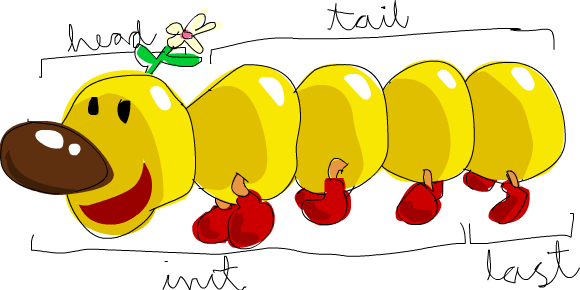
\includegraphics[height=2\baselineskip]{./listmonster.png}
\end{wrapfigure}
\haskellinline{head[1,2,3] => 1}, \haskellinline{tail[1,2,3] => [2,3]}\\
\haskellinline{init [1,2,3] => [1,2]}, \haskellinline{last [1,2,3] => 3}\\
\haskellinline{take n l -- erste n Elemente von l}\\
\haskellinline{drop n l  -- l ohne erste n Elemente}\\

\noindent
\haskellinline{takewhile bedingung liste}\\
\haskellinline{dropwhile bedingung liste}\\
\haskellinline{span b l == (takewhile b l, dropwhile b l)}\\

\noindent
\haskellinline{null[1,2,3] => False}\\
\haskellinline{length}\\
\haskellinline{isIn}
\begin{minted}{haskell}
a ++ b
xs !! n -- Nte Listenelement
reverse xs
map f (x:xs) -- wendet f auf alle Listenelemente an
filter pred (x:xs) -- behalte alle Elemente, die Prädikat erfüllen
\end{minted}
\subsection{Funktionsanwendungen}\label{subsec:funktionsanwendungen}
Funktionskomposition $f \circ g$: \haskellinline{comp f g = (\x -> f (g x))} Infix: \haskellinline{f.g}\\
n-Fache Funktionsanwendung $f^n$: \haskellinline{iter f n}\\
\textcolor{darkgray}{Funktionstypen sind rechts-assoziativ, Funktionsanwendung ist links-assoziativ}\\
\haskellinline{f x = y + x} Variable $x$ Gebunden, Variable $y$ frei.\\
\subsection{Lokale Namensbindung}\label{subsec:lokale-namensbindung}
\begin{multicols}{2}
    \begin{minted}{haskell}
energy m = let c = 299
        square = x = x * x
    in m * (square c)
    \end{minted}
\columnbreak
    \begin{minted}{haskell}
energy m = m * (square c)
    where c = 299
        square x = x * x
    \end{minted}
\end{multicols}
\textcolor{darkgray}{Einrückung hat semantische Bedeutung}.\\
\textcolor{darkgray}{Bei Schachtelung: Inneres \haskellinline{let} bindet stärker.}\\
\subsection{Folds}\label{subsec:folds}
%! suppress = Ellipsis
\begin{minted}[escapeinside=||]{haskell}
foldr operator initial [] = initial
foldr operator initial (x:xs) = operator x (foldr operator initial xs)
|\textcolor{darkgray}{\texttt{foldr f z [x1, x2, \ldots, xn] == x1 `f` (x2 `f`\ldots(xn `f` z)\ldots)}}|
foldl op i [] i
foldl op i (x:xs) = foldl op (op i x) xs
|\textcolor{darkgray}{\texttt{foldl f z [x1, x2, \ldots, xn] == (\ldots((z `f` x1) `f` x2) `f`\ldots)`f` xn}}|
\end{minted}
\textcolor{darkgray}{Beispiel: \texttt{length \sout{list} = foldr (\textbackslash x n -> n + 1) 0 \sout{list}}}
\begin{multicols}{2}
\begin{minted}{haskell}
concat [xs, ys, zs] = xs ++ ys ++ zs
\end{minted}
\columnbreak
\textcolor{darkgray}{\texttt{concat == foldr app []}}
\end{multicols}
\begin{minted}{haskell}
zipWith f (x:xs) (y:ys) = f x y : zipWith f xs ys
zipWith f xs ys = []
zip = zipWith (,) -- zip[1,2,3],[7,8,9] = [(1,7),(2,8),(3,9)]
\end{minted}
Kurznotation Intervalle \haskellinline{[a..b]} $=>^+$ \haskellinline{[a, a+1, a+2, ..., b]}\\
List Comprehensions \haskellinline{[e | q1, ..., qm]}, $q_i$ Tests oder Generatoren der Form $p \leftarrow list$ mit Muster $p$ und Listenausdruck $list$\\
\textcolor{darkgray}{Beispiel: \texttt{squares n = [x * x | x <- [0..n]]}}\\
Im Muster \texttt{p} gebundene Variablen können in \texttt{e} und in \texttt{qi} verwendet werden\\
%! suppress = RedundantEscape
\textcolor{darkgray}{Beispiel: \texttt{evens n = [x | $\underbrace{\texttt{x<-[0..n]}}_\text{Generator}$, $\underbrace{\texttt{x \textasciigrave mod \textasciigrave 2 == 0]}}_\text{Tester}$}}\\
\textbf{Unendliche Listen}: \haskellinline{odds = 1 : map (+2) odds}
%! suppress = LineBreak
\begin{minted}[escapeinside=||]{haskell}
iterate f a = a : iterate f (f a)
|\textcolor{darkgray}{odds = iterate (+2)  1}|
iterate f x !! 23 -- führt "Schleife" 23 mal aus
\end{minted}
\subsection{Typen}\label{subsec:typen}
\begin{minted}[escapeinside=||]{haskell}
type neuerName = [Integer]
               = String
               = (a, b)
               = |\dots|
\end{minted}
\begin{multicols}{2}
Algebraische Datentypen
\begin{minted}{haskell}
data Shape = Circle Double
        | Rectangle Double Double
\end{minted}
\columnbreak
Konstruktoren
\begin{minted}{haskell}
Circle :: Double -> Shape
Rectangle :: Double -> Double -> Shape
\end{minted}
\end{multicols}
Aufzählungstypen
\begin{minted}{haskell}
data Season = Spring | Summer | Autumn | Winter
\end{minted}
Polymorphe Datentypen (Optionale Werte)
\begin{minted}{haskell}
data Maybe t = Nothing | Just t
data Either s t = Left s | Right t
data Matrix t = Dense [[t]] -- Liste von Zeilen
        | Sparse [(Integer, Integer t)] t -- Einträge (i,j,v) und Defaultwert
data Stack t = Empty | Stacked t (Stack t)
\end{minted}
Polymorphe Funktion mit Typeinschränkung
\begin{multicols}{2}
\begin{minted}[escapeinside=||]{haskell}
qsort :: Ord t => [t] -> [t]
qsort [] = []
qsort (p:ps) = |\dots|
\end{minted}
\columnbreak
Instanzen von Ord implementieren \haskellinline{<=, <, >, >=, ...}
\end{multicols}
\begin{multicols}{2}
Typklassen-Definitionen
\begin{minted}[escapeinside=\{\}]{haskell}
instance Eq Bool where
    True == True = True
    True == False = False
          {\vdots}
    \end{minted}
    \columnbreak
    Fehlende Implementierungen: Default implementiert
\end{multicols}
\begin{minted}{haskell}
data shape = Circle Double
        | Rectangle Double Double
        deriving Eq -- Keine eigene (==) Funktion mehr notwendig
\end{minted}
Automatische Instanziierung auch für \haskellinline{Show},\haskellinline{Ord},\haskellinline{Enum}
\subsection{Monaden}\label{subsec:monaden}
\newpage
\section{λ-Kalkül}\label{sec:lambda-kalkul}
\subsection{untypisiertes λ-Kalkül}\label{subsec:untypisiertes-lambda-kalkul}
\begin{table}[H]
    \centering
    \begin{tabular}{llll}
        \toprule
        \textbf{} & \textbf{Notation} & \textbf{Beispiele}\\
        \midrule
        Variablen & $x$ & $x$ & $y$ \\
        Abstraktion & $\lambda x.t$ & $\lambda y.0$ & $\lambda f.\lambda x. \lambda y.f\ y\ x$ \\
        Funktionsanwendung & $t_1 t_2$ & $f 42$ & $\lambda x.x + 5)\ 7$ \\
        \bottomrule
    \end{tabular}
    \label{tab:table}
\end{table}
Funktionsanwendung linksassoziativ, bindet stärker als Abstraktion
\begin{table}[H]
    \centering
    \begin{tabularx}{\textwidth}{lX}
        \textalpha-Äquivalenz & $t_1$ und $t_t$ heißen \textalpha-äquivalent $t_1\stackrel{\alpha}{=}t_2$, wenn $t_1$ in $t_2$ durch konsistente Umbenennung der \textlambda-gebundenen Variablen überführt werden kann\\
        \texteta-Äquivalenz & Terme $\lambda x.f\ x$ und $f$ heißen \texteta-äquivalent ($\lambda x.f\ x\stackrel{\eta}{=}f$) falls $x$ nicht freie Variable vob $f$\\
        Redex & Ein \textlambda-Term der Form $(\lambda x.t_1)\ t_2$ heißt Redex\\
        \textbeta-Reduktion & \textbeta-Reduktion entspricht der Ausführung der Funktionsanwendung auf einen Redex \[(\lambda x.t_1)t_2 \Rightarrow t_1 [x\mapsto t_2]\]\\
        Substitution & $t_1[x\mapsto t_2]$ erhält man aus den Term $t_1$, wenn man alle freien Vorkommen von $x$ durch $t_2$ ersetzt\\
        Normalform & Ein Term, der nicht weiter reduziert werden kann\\
        Volle \textbeta-Reduktion & Jeder Redex kann jederzeit reduziert werden\\
        Normalreihenfolge & Immer der linkeste äußerste Redex wird Reduziert\\
    \end{tabularx}
    \label{tab:2}
\end{table}
$let\ x = t_1\ in\ t_2$ wird zu $(\lambda x.t_2)\ t_1$
\subsection{Church-Zahlen}\label{subsec:church-zahlen}
Eine (natürliche) Zahl drückt aus, wie oft die funktion $s$ angewendet wurde\\
    \begin{multicols}{2}
        \begin{equation*}
            \begin{aligned}
                c_0 &= \lambda s.\lambda z.z\\
                c_1 &= \lambda s.\lambda z.s\ z\\
                c_2 &= \lambda s. \lambda z.s\ (s\ z)\\
                &\vdots\\
                c_n &= \lambda s. \lambda z\ s^n\ z
        \end{aligned}\label{eq:equation}
        \end{equation*}
        \columnbreak\\
        Nachfolgefunktion \[succ = \lambda n.\lambda s.\lambda z.s\ (n\ s\ z)\]
        wobei $n$ Church Zahl
    \end{multicols}
\begin{table}[H]
    \centering
    \begin{tabularx}{\textwidth}{lX}
        Addition & $plus = \lambda m.\lambda n.\lambda z.m\ s\ (n\ s\ z)$\\
        Multiplikation & $\begin{aligned} times &= \lambda m.\lambda n.\lambda s.n(m\ s)\\&\stackrel{\eta}{=} \lambda m.\lambda n.\lambda s.\lambda z.n(m\ s)\ z\end{aligned}$\\
        Potenzieren & $\begin{aligned} exp &= \lambda m.\lambda n.n\ m\\&\stackrel{\eta}{=}\lambda m.\lambda n.\lambda s.\lambda z.n\ m\ s\ z\end{aligned}$\\
    \end{tabularx}\label{tab:table2}
    \begin{tabularx}{\textwidth}{ll}
        $c_{true}= \lambda t.\lambda f.t$ & $c_{false} = \lambda t.\lambda f.f$\\
    \end{tabularx}
    \begin{tabularx}{\textwidth}{l}
    $isZero = \lambda n.n\ (\lambda x.c_{false})\ c_{true}$
    \end{tabularx}
\end{table}
\noindent
    Rekursionsoperator
    $Y =\lambda f.(\lambda x.f\ (x\ x))(\lambda x.f\ (x\ x))$\\
    $f\ (Y\ f)\stackrel{\eta}{=}Y\ f$\\
    $Y\ f$ ist Fixpunkt von $f$\\

\noindent
    Church-Rosser: Wenn $t \Rightarrow t_1$ und $t_1 \stackrel{*}{\Rightarrow} t_2$, dann gibt es $t'$ mit $t_1 \stackrel{*}{\Rightarrow}t'$ und $t_2 \stackrel{*}{\Rightarrow}t'$
    \begin{table}[H]
        \centering
        \begin{tabularx}{\textwidth}{lX}
            Call-by-name & Reduziere linkesten äußersten Redex aber nicht, falls von einem \textlambda\ umgeben \textrightarrow\ Reduziere Argumente erst, wenn benötigt\\
            Call-by-Value & Reduziere linkesten Redex, der nicht von einem \textlambda\ umgeben und dessen Argument ein Wert \textrightarrow\ Argument vor Funktionsaufruf ist auszuwerten\\
        \end{tabularx}\label{tab:table3}
    \end{table}
\subsection{Regelsysteme}\label{subsec:regelsysteme}
Fregescher Schlussstrich
\begin{equation*}
    \typeRule{}{
    \varphi_1\quad\varphi_2\quad\varphi_3\quad...\quad\varphi_n
    }{
    \varphi
    }
\end{equation*}
Jede Regel stellt Implikation dar, $\varphi_i$ Voraussetzungen, $\varphi$ Konklusion\\

\begin{table}[H]
    \centering
    \begin{tabularx}{\textwidth}{lXX}
        & \centerline{\textbf{Introduktionsregel}} &\centerline{\textbf{Eliminationsregel}}\\
        Konjunktion &\begin{equation*}\typeRule{$\wedge{}I$}{\psi\ \varphi}{\psi\wedge \varphi}\end{equation*}&\begin{equation*}\typeRule{$\wedge{}E_1$}{\psi\wedge \varphi}{\psi}\quad\typeRule{$\wedge{}E_2$}{\psi\wedge \varphi}{\varphi}\end{equation*}\\
        All-Quantor &\begin{equation*}\typeRule{$\forall{}I$}{P(y)\ y\ ist\ frei\ in\ P}{\forall{}x.P(x)}\end{equation*}&\begin{equation*}\typeRule{$\forall{}E$}{\forall{}x.P(x)}{P(y)}\end{equation*}\\
        Implikation&\begin{equation*}\typeRule{$\rightarrow{}I$}{\begin{aligned}&\psi&\\&\vdots\footnotemark{}&\\&\varphi&\end{aligned}}{\psi\longrightarrow\varphi}\end{equation*}&\begin{equation*}\typeRule{MP}{\psi\longrightarrow\varphi\quad\psi}{\varphi}\end{equation*}\\
    \end{tabularx}\label{tab:table4}
\end{table}
\footnotetext{Herleitung gemäß Regeln verbindet Implikation der Regeln mit prädikatenlogischer Implikation}

Alternative Notation
\begin{equation*}
    \typeRule{}{
    \Gamma_1 \vdash \varphi_1\quad\dots\quad\Gamma_n\vdash\varphi_n
    }{
    \vdash \varphi
    }
\end{equation*}
Regelsysteme alternative Notation
\begin{table}[H]
    \centering
    \begin{tabularx}{\textwidth}{XX}
        \centerline{\textbf{Introduktionsregeln}} &\centerline{\textbf{Eliminationsregeln}}\\
        \begin{equation*}\typeRule{$\wedge{}I$}{\Gamma\vdash\varphi\quad\Gamma\vdash\psi}{\Gamma\vdash\varphi\wedge\psi}\end{equation*}&\begin{equation*}\typeRule{$\wedge{}E_1$}{\Gamma\vdash\psi\wedge\psi}{\Gamma\vdash\varphi}\quad\typeRule{$\wedge{}E_2$}{\Gamma\vdash\varphi\wedge\psi}{\Gamma\vdash\psi}\end{equation*}\\
        \begin{equation*}\typeRule{$\rightarrow{}I$}{\Gamma,\varphi\vdash\psi}{\Gamma\vdash\varphi\longrightarrow\psi}\quad\typeRule{AssmI}{}{\Gamma,\varphi\vdash\varphi}\end{equation*}&\begin{equation*}\typeRule{MP}{\Gamma\vdash\varphi\longrightarrow\psi\quad\Gamma\vdash\varphi}{\Gamma\vdash\psi}\end{equation*}\\
        \begin{equation*}\typeRule{$\wedge{}I_1$}{\Gamma\vdash\varphi}{\Gamma\vdash\varphi\wedge\psi}\quad\cdots\end{equation*}&\begin{equation*}\typeRule{VE}{\Gamma\vdash\varphi\wedge\psi\quad\Gamma,\varphi\vdash\omega\quad\Gamma,\psi\vdash\omega}{\Gamma\vdash\omega}\end{equation*}\\
    \end{tabularx}\label{tab:table5}
\end{table}
\newpage
\subsection{Typsysteme}
Funktionstypen rechtsassoziativ
Typsystem $\Gamma\vdash t:\tau$ im Typkontext $\Gamma$ hat Term $t$ Typ $\tau$. $\Gamma$ ordnet freien Variablen $x$ ihren Typ $\Gamma(x)$ zu.
\begin{table}[H]
    \centering
    \begin{tabularx}{\textwidth}{XX}
        \begin{equation*}\typeRule{Const}{c \in Const}{\Gamma\vdash{}c:\tau_2}\end{equation*}&\begin{equation*}\typeRule{Var}{\Gamma(x)= \tau}{\Gamma\vdash{}x:\tau}\end{equation*}\\
        \begin{equation*}\typeRule{Abs}{\Gamma,x:\tau_1\vdash{}t:\tau_2}{\Gamma\vdash\lambda{}x.t:\tau_1\longrightarrow\tau_2}\end{equation*}&\begin{equation*}\typeRule{App}{\Gamma\vdash{}t_1:\tau_2\longrightarrow\tau\quad\Gamma\vdash{}t_2:\tau_2}{\Gamma\vdash{}t_1\ t_2:\tau}\end{equation*}\\
        \end{tabularx}\label{tab:table6}
\end{table}
Typisierung von \textlambda{}-Term $t$: Paar $(\Gamma,\tau)$, sodass $\Gamma\vdash{}t:\tau$ herleitbar\\
\textcolor{darkgray}{\textbeta-Reduktion: Substitution von x $(\lambda{}x.t_1)\ t_2 \Rightarrow t_1[x\mapsto t_2]$}
\begin{table}[H]
    \centering
    \begin{tabularx}{\textwidth}{lX}
        Substitutionslemma & Wenn $\Gamma,x:\tau_2\vdash{}t_1:\tau_1$ und $\Gamma\vdash{}t_2:\tau_2$ dann $\Gamma\vdash{}t_1[x\mapsto{}t_2]:\tau_1$\\
        Typerhaltungstheorem & Wenn $\Gamma\vdash{}t:\tau$ und $t\Rightarrow{}t'$ dann $\Gamma\vdash{}t':\tau$\\
        Typschema & Typ der Gestalt $\forall\alpha_1.\forall\alpha_2.\cdots\forall\alpha_n$ heißt Typschema.
        Es bindet freie Typvariablen $\alpha_1\dots\alpha_n$ in $\tau$\\
        Instanziierung eines Typschemas & Für nicht-Schema-Typen $\tau_2$ ist der Typ $\tau[\alpha\mapsto\tau_2]$ eine Instanzieierung vom Typschema $\forall\alpha.\tau$\\
        &Schreibweise $(\forall\alpha.\tau)\succeq\tau[\alpha\rightarrow\tau_2]$\\
        \textcolor{darkgray}{Beispiele} & \textcolor{darkgray}{$\forall\alpha.\alpha\rightarrow\alpha\succeq{}int\rightarrow{}int$}\\
        &\textcolor{darkgray}{$\forall\alpha.\alpha\rightarrow\alpha\succeq{}(int\rightarrow{}int)\rightarrow(int\rightarrow{}int)$\quad$int\succeq{}int$}\\
        &\textcolor{darkgray}{$\alpha\rightarrow\alpha\nsucceq{}int\rightarrow{}int$\quad$\alpha\nsucceq{}bool$}\\
        &\textcolor{darkgray}{$\forall\alpha.\alpha\rightarrow\alpha\nsucceq{}bool$}\\
    \end{tabularx}
    \label{tab:3}
\end{table}
\newpage
\subsection{Typinferenz}\label{subsec:typinferenz}
    \begin{table}[H]
        \centering
        \begin{tabularx}{\textwidth}{X|X}
            \begin{equation*}\begin{aligned}\typeRule{Var}{\Gamma(x)=\sigma\quad\sigma\succeq\iota}{\Gamma\vdash{}x:\tau} \\ \text{Constraint: }\{\iota=\tau\}\end{aligned}\end{equation*}&\begin{equation*}\begin{aligned}\typeRule{App}{\Gamma\vdash{}f:\xi\quad\Gamma\vdash{}x:\varphi}{\Gamma\vdash{}f\ x:\alpha}\\ \text{Constraint: }\{\xi=\varphi\rightarrow\alpha\}\end{aligned}\end{equation*}\\
            \hline
            \begin{equation*}\begin{aligned}\typeRule{Abs}{\Gamma,p:\pi\vdash{}b:\beta}{\Gamma\vdash\lambda{}p.b:\alpha}\\ \text{Constraint: }\{\alpha=\pi\rightarrow\beta\}\end{aligned}\end{equation*}&\begin{equation*}\begin{aligned}\typeRule{Let}{\Gamma\vdash{}y:\pi\quad\Gamma'\vdash{}b:\beta}{\Gamma\vdash\mylet{x}{y}{b:\tau}}\\ \text{Constraints: Siehe unten}\end{aligned}\end{equation*}\\
        \end{tabularx}\label{tab:table7}
    \end{table}
    $ta(\tau,\Gamma)$ bindet alle in $\Gamma$ freien Typvariablen mit einem $\forall$ in $\tau$\\
    Bsp.: $ta(\alpha\rightarrow\beta,x:\beta,y:\delta)=\forall\alpha.\alpha\rightarrow\beta$
    \begin{equation*}
        \typeRule{Let}{\Gamma\vdash{}y:\pi\quad\Gamma'\vdash{}b:\beta}{\Gamma\vdash\mylet{x}{y}{b:\tau}}
    \end{equation*}
    Constraints: Finde Unifikator $\sigma_\textsc{let}$ und allg. Typ $\pi$ für $y$
    \begin{enumerate}
        \item Sei $C_0$ die bisherige Constraintmenge inklusive $\{\tau=\beta\}$
        \item Sammle Constraints aus linken Teilbaum in $C_\textsc{let}$
        \item Berechne \textit{mgu} $\sigma_\textsc{let}$ von $C_\textsc{let}$
        \item Berechne $\Gamma':=\sigma_\textsc{let}(\Gamma),x:ta(\sigma_\textsc{let}(\pi),\sigma_\textsc{let}(\Gamma))$
        \item Benutze $\Gamma'$ in rechten Teilbaum, sammle Constraints in $C_1$
        \item Ergebnisscontraints sind $C_0\cup{}C'_\textsc{let}\cup{}C_1$\\
        mit $C'_\textsc{let} := \{\alpha_i = \sigma_\textsc{let}(\alpha_i)|\sigma_\textsc{let}$ definiert für $\alpha_i\}$
    \end{enumerate}
    \textcolor{darkgray}{
    Typen sind Rechstassoziativ also wenn suche nach mgu und
    \begin{equation*}
        \begin{aligned}
            \alpha_1&=\alpha_3\rightarrow\alpha_4\rightarrow\alpha_5  = (\alpha_3\rightarrow(\alpha_4\rightarrow\alpha_5))\\
            \alpha_2&=\alpha_6\rightarrow\alpha_7\\
            \text{dann}\\
           \alpha_6&\text{ \pointer\ }\alpha_3\\
            \alpha_7&\text{ \pointer\ }\alpha_4\rightarrow\alpha_5
        \end{aligned}
    \end{equation*}
    }
%\begin{equation*}
%    \typeRule{Abs}{
%    ... \vdash ...
%    }{
%    \vdash \abs{x}{\abs{y}{\liin{y}{\lii{x}{y}}}} : ((\alpha \to \beta) \to \alpha) \to (\alpha \to \beta) \to \beta
%    }
%\end{equation*}
%
% BibTeX Literaturverzeichnis
%
\section{Handschrift}
Ziel dieses Dokumentes war es  die handschriftliche Zusammenfassung abzutippen. Leider war das \emph{wesentlich} schwieriger und zeitaufwändiger als gedacht.\\
Deswegen \enquote{for completeness Sake} im folgenden die Handschriftliche version auf der diese Zusammenfassung basiert
\clearpage
\includepdf[pages=-]{Propa_Handschrift}
\end{document}
